\section{Implementation}

The Anastasis is written in C. We decided to use C because of the
various dependencies, including cryptographic libraries.  Especially,
GNU Taler and Sync, which are working in concert with Anastasis, are
also written in C. Using the same language makes integration and
testing of Anastasis much easier.

The whole Anastasis application consists of multiple components.
Figure~\ref{fig:secret_split:overview} gives an overview over all the
components.

\begin{figure}[H]
	\centering
		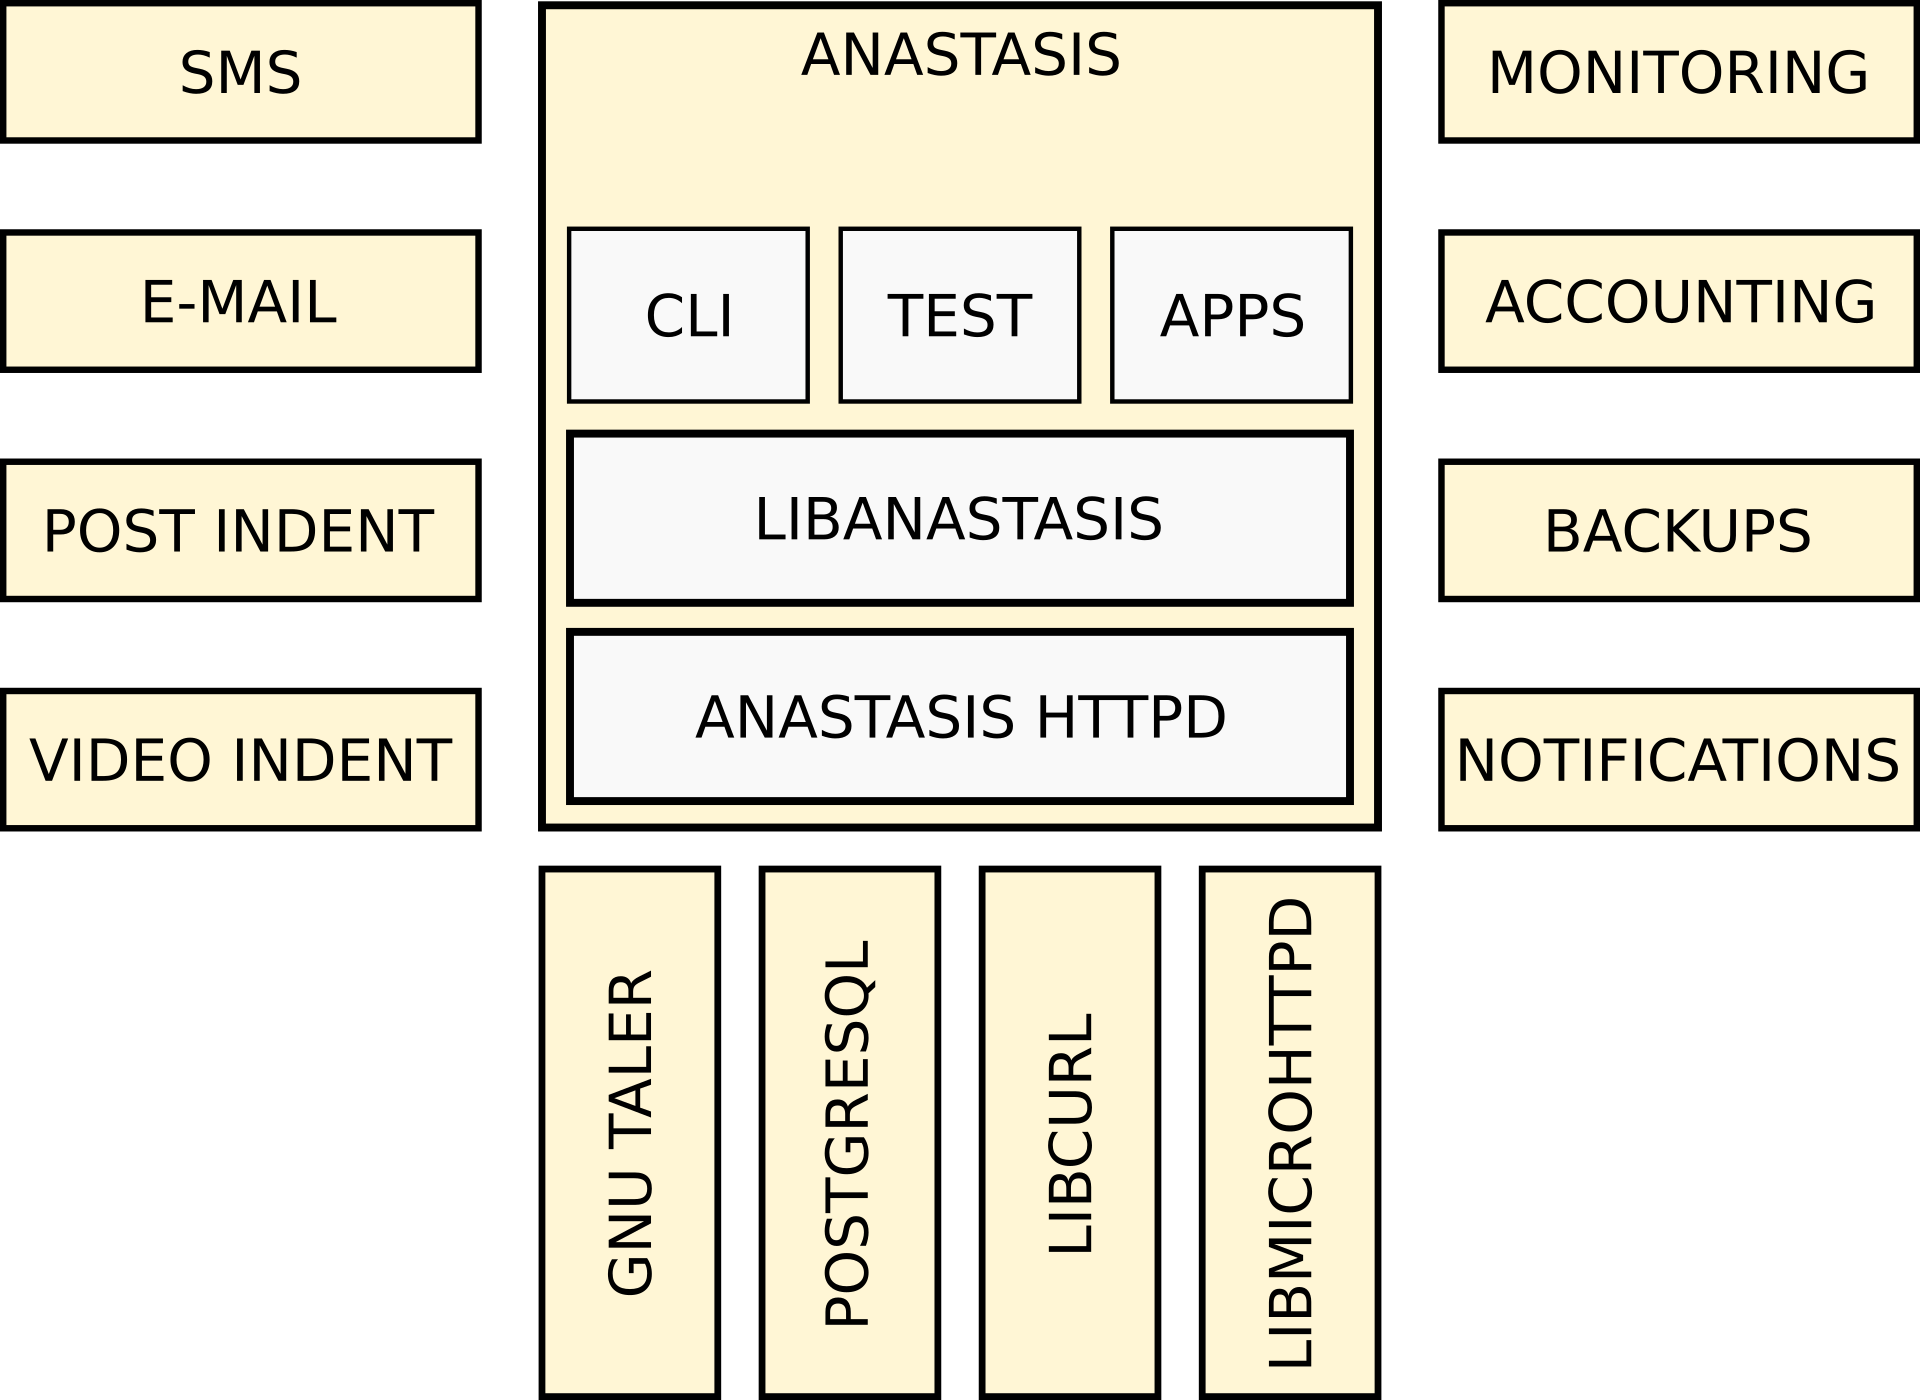
\includegraphics[scale=0.5]{images/system-architecture.png}
	\caption{System architecture overview}
	\label{fig:system_arch:overview}
\end{figure}

\noindent In the center is the core implementation of Anastasis.
On the left are some of the planned authentication methods from the
application. On the right side of the box are the core parts which are
necessary to operate Anastasis commercially. These parts are
anticipated for a production deployment, but not part of the
implementation for this thesis.

At the bottom section are the external libraries used for the project.
These libraries are presented in Section~\ref{sec:libraries}.
\newpage


\subsection{System architecture}

This graphic shows the basic architecture of the Anastasis
application. It shows a simplified flow of the application. The
details of each component are explained later.

\begin{figure}[H]
	\centering
		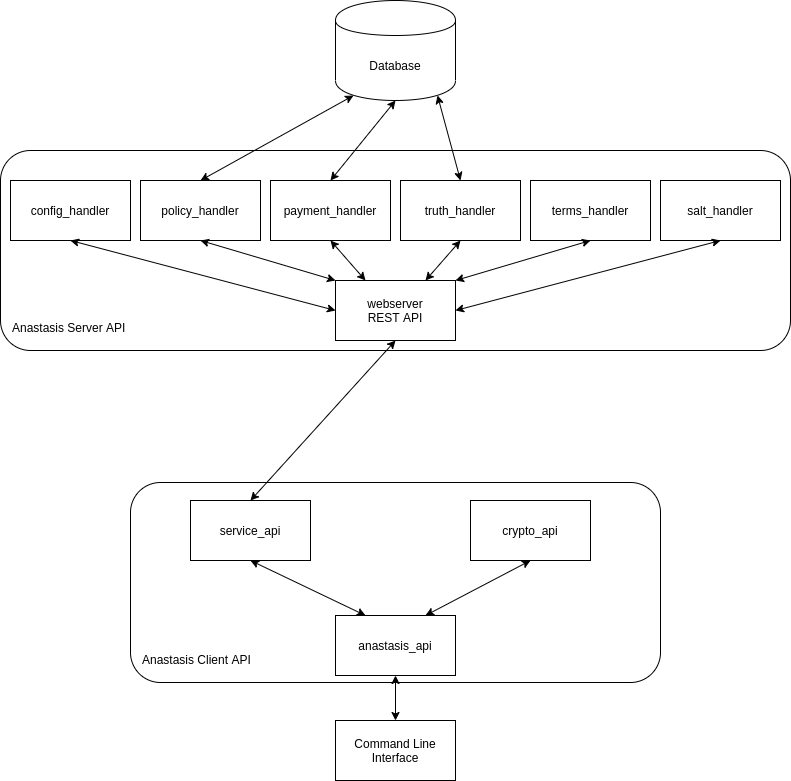
\includegraphics[scale=0.4]{images/system_design.png}
	\caption{System design overview}
	\label{fig:system_design}
\end{figure}

\begin{enumerate}
\item The Anastasis CLI interacts with the Anastasis API. The
  Anastasis API is responsible for triggering interactions with the
  user, and also manages the interactions between the
  various client-side components.
\item After the user provided their unforgettable secret, the
  Crypto API derives the needed key material for the further
  communication. This is simplified, in reality the client would first
  need to download the server salt to generate the user keys.  The
  crypto API is later also responsible for the decryption and
  encryption of the data, sent or received from the server.
\item The Service API is responsible for the communication with the
  Anastasis server. The Anastasis API sends the previously generated
  data and the user selected request to the service.
  The Service API is also responsible to handle
  the server's response to the request.
\item The central webserver logic handles HTTP requests sent to it by the
  clients. It will dispatch requests to the corresponding handler. The
  webserver's core logic also returns the response and the status code
  of the operation to the client application.
\item Each REST endpoint of the Anastasis server is implemented by
  a specific handler. The handler processes the requests, typically
  by storing or looking up the requested
  data with the database. When the request is finished, the handler will
  send back the data or the status code to the webserver's core logic.
\end{enumerate}


\subsection{Server architecture} \label{sec:serverarch}

The Anastasis server architecture consists of two components. A web
server with a REST API and a PostgreSQL database. The structure of
these two components is shown in Figure~\ref{fig:anastasis:server}.

\begin{figure}[H]
	\centering
	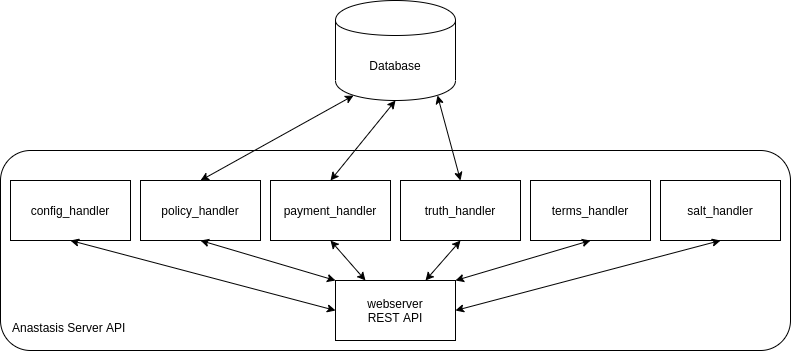
\includegraphics[scale=0.45]{images/server_api.png}
	\caption{Anastasis server architecture}
	\label{fig:anastasis:server}
\end{figure}

The webserver of Anastasis provides a RESTful API. For a detailed
documentation of the REST API, see
appendix ~\ref{appendix_server_api}.

\newpage
\subsubsection{Database}

The database schema of Anastasis is shown in
Figure~\ref{fig:anastasis_database}.
\begin{figure}[H]
	\centering
	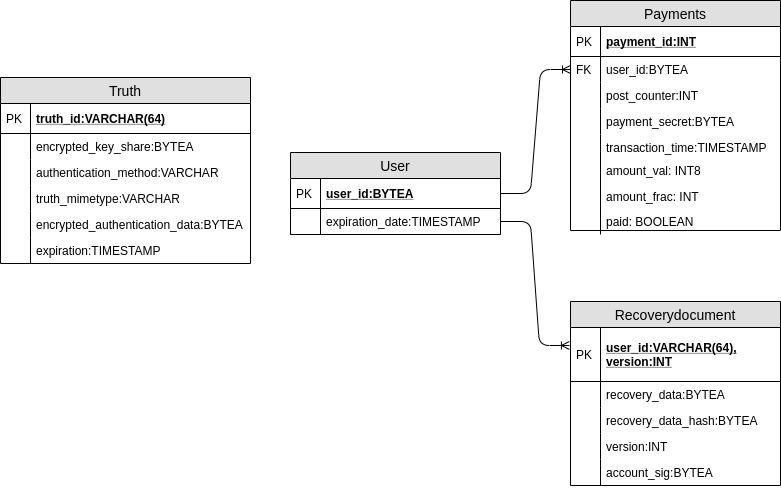
\includegraphics[scale=0.5]{images/anastasis-db.png}
	\caption{Anastasis database schema}
	\label{fig:anastasis_database}
\end{figure}

The database schema consists of four main tables:

\begin{itemize}
\item The {\em Truth} table is responsible for storing the key shares and
  its authentication method. The key share and the authentication data are stored
  encrypted in the database. The authentication data is only decrypted during
  authentication. The key share is never decrypted for the
  server. This protects the privacy of the customer. Likewise, the
  user data is protected after a possible theft.
\item The {\em User} table contains the identification of the user and an
  expiration timestamp. This timestamp is a subscription period. This
  timestamp is updated after each payment the user makes. Users for
  whom the subscription has expired are periodically deleted.
\item The {\em Payments} table contains the details of a payment from a
  user. The payment is used either for the post-counter or the
  subscription. The post-counter is decremented after each upload of a
  recovery document. The user can only upload the recovery document if
  the provided payment contains a post-counter which is at least 1.
  Through this measure we can prevent people from maliciously filling
  our database.
\item The {\em Recoverydocument} table contains the recovery
  information. The recovery document is stored encrypted in the
  database. This offers better protection, as explained earlier for
  the Truth table. Each recovery document record also contains a
  version, a hash of the recovery document and a signature. The
  version attribute allows the user to lookup a specific version of
  the document. The hash is used to check if the user uploads a
  duplicate of the document. The signature attests the
  integrity of the recovery data.
\end{itemize}


\subsubsection{Authentication methods}

This section describes an overview over the different possible
authentication methods for Anastasis. In our implementation only the
secure question is implemented. The other methods are just explained
how they would be implemented.

In all cases, the authentication process begins by the user decrypting
their (encrypted) recovery document, which contains a list of Anastasis
providers, associated authentication methods, truth\_seeds and associated
truth encryption keys.  The recovery process than varies slightly
depending on the authentication method.

\paragraph{SMS (sms)}

The user tells the server with a request that they wants to authorize
key recovery (via GET /truth/\$TRUTH\_PUB), providing a way to decrypt the
truth with the phone number. The server will then generate a \$PIN and
send it via an SMS provider to the stored number in the truth
object. The client then must send another request with the sent \$PIN
(via GET /truth/\$TRUTH\_PUB?response=\$PIN). The server can now check
if the two PINs match. Upon success, the server returns the encrypted
key share.

\paragraph{Video identification (vid)}

This method allows the user to identify via video-call.  Since the
respective images must be passed on to the video identification
service in the event of password recovery, it must be ensured that no
further information about the user can be derived from them.  Hence,
the user's client software must try to delete metadata that could
result in accidental information leakage about the user from the image
before encrypting and uploading it to the Anastasis provider.

For recovery, the user must first send a request to server that they
wants to authorize recovery (GET /truth/\$TRUTH\_PUB).  The Anastasis
provider will then decrypt the user's image and send a request with a
\$TOKEN to a video authentication provider that a user wants to
authenticate, and respond to the user with a link to a video
conference.  The video authentication provider then checks via video
conference that the user in the image is the same that they have on
the video link. Upon success, the video provider releases the \$TOKEN
to the user.  The client then must send another request with the
\$TOKEN (via GET /truth/\$TRUTH\_PUB?response=\$TOKEN). The Anastasis
provider checks that the tokens match, and upon success returns the
encrypted key share.

\paragraph{Post identification (post)}

The user tells the Anastasis provider with a request that they want
to authenticate using Post identification (GET /truth/\$TRUTH\_PUB).  The
Anastasis provider uses the request to decrypt the user's truth to
determine the user's postal address, and sends them letter containing
a \$PIN.  Upon receiving the letter, the client then has to send
another request with the \$PIN (GET /truth/\$TRUTH\_PUB?response=\$PIN). The
server can now check if the two PINs match. Upon success the server
will release the encrypted key share.

\paragraph{Security question (qa)}

The user provided Anastasis with a secure question and a (normalized)
answer.  The secure question becomes part of the encrypted recovery
document, and is never disclosed to weak adversaries, even during
recovery.  The encrypted truth on the server only contains a (salted)
hash of the answer. The Anastasis provider cannot learn the plaintext
answer. Because of the salt, and it cannot mount a confirmation attack
either.

If the user wants to recover the key share from the server, they must
provide the (salted) hash of the answer to the security question (via
GET /truth/\$TRUTH\_PUB?response=\$HASH). The server then checks if the
stored and the provided hash match. Upon success the server responds
with the encrypted key share.


\subsection{Client architecture}

The Anastasis client architecture consists of two main components. A client
API which communicates with the server and a command line application
which interacts with the user. The structure of these two components
is shown in Figure~\ref{fig:anastasis:client}.

\begin{figure}[H]
	\centering
	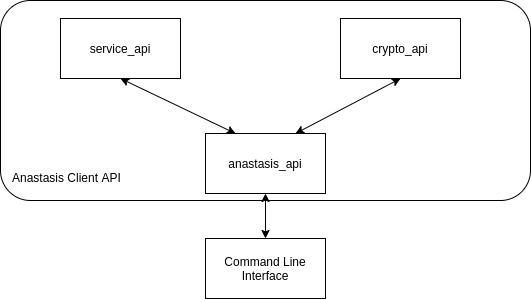
\includegraphics[scale=0.6]{images/client_api.png}
	\caption{Anastasis client architecture}
	\label{fig:anastasis:client}
\end{figure}

The Anastasis client implementation includes three distinctive APIs: a
{\em Crypto API} which provides the different cryptographic functions,
a {\em Service API} which sends the request to the server and the {\em
  Client API} which manages the main data structures and provides an
abstraction for the application.

\subsubsection{Crypto API}

The most important data structures in the crypto API are the following:

\begin{itemize}
  \item
The kdf\_id is a hash code which was generated with Argon2. The
entropy source is the user's unforgettable secret. The kdf\_id is used
to create various key's, for more details see Chapter~\ref{chap:design}.

\begin{lstlisting}
struct kdf_id
{
  Hashcode; //512-bit
}
\end{lstlisting}

\item
The account\_private\_key is used to sign the data and check the signature later. It is a 256-bit EdDSA private key. It is generated with the kdf\_id as entropy source.
\begin{lstlisting}
struct account_private_key
{
  eddsa_private_key;
}
\end{lstlisting}

\item
The account\_public\_key is used as the user identification on the different providers. It is generated from the private\_key.
\begin{lstlisting}
struct account_public_key
{
  eddsa_public_key;
}
\end{lstlisting}

\item
The truth\_key is a randomly generated AES-256 GCM key. It is used to encrypt the user specify data in the truth object.
\begin{lstlisting}
struct truth_key
{
  key; //256-bit
}
\end{lstlisting}

\item
The truth\_seed is a randomly generated nonce with a size of 32 Bytes. It is used to derive a truth\_private\_key
and is stored within an encrypted recovery document.
\begin{lstlisting}
struct truth_seed
{
  nonce; //256-bit
}
\end{lstlisting}

\item
The truth\_private\_key is used to sign the encrypted key share and the encrypted authentication data. It is a 256-bit EdDSA private key. It is generated with the truth seed as entropy source.
\begin{lstlisting}
struct truth_private_key
{
   eddsa_private_key;
}
\end{lstlisting}

The truth\_public\_key is used as the user identification on the different providers in case of uploaded truths. It is generated from the truth private key.
 \begin{lstlisting}
struct truth_public_key
{
  eddsa_public_key;
}
\end{lstlisting}


\item
Anastasis needs different symmetric keys to encrypt data for example, the recovery document. These symmetric keys are all 256-bit large hashcodes. These symmetric keys are generated through the key routine defined in Implementation Key usage.
\begin{lstlisting}
struct symmetric_key
{
  hashcode; //256-bit
}
\end{lstlisting}

\item
Each policy has a separate policy\_key. The key is used to encrypt the master\_key.
The policy\_key is also a AES-256 GCM key. It is generated through the combination of a set of key\_shares.
\begin{lstlisting}
struct policy_key
{
  hashcode; //256-bit
}
\end{lstlisting}

\item
Every truth object contains a key\_share. A key\_share is a 256-bit random generated bit sequence.
\begin{lstlisting}
struct key_share
{
  hashcode; //256-bit
}
\end{lstlisting}

\item
Before every encryption a random 256-bit large nonce is generated. This gives the encryption algorithm a random factor.
\begin{lstlisting}
struct nonce
{
  hashcode; //256-bit
}
\end{lstlisting}

\item
To use AES-256 GCM an IV must be generated. It is generated with an HKDF over a salt the kdf\_id and a symmetric key.
\begin{lstlisting}
struct iv
{
  hashcode; //128-bit
}
\end{lstlisting}

\item
The aes\_tag is generated after each encryption, it is later used to check the integrity of the data.
\begin{lstlisting}
struct aes_tag
{
  hashcode; //128-bit
}
\end{lstlisting}
\end{itemize}

The functions of the crypto API basically provide the canonical set of
cryptographic operations (hash, encrypt, decrypt, etc.)  over these
basic data structures.


\subsubsection{Client API}

The most important data structures in the client API are the following:

\begin{itemize}
  \item
The secret share data structure is used to upload a new recovery document.
\begin{lstlisting}
struct secret_share
{
  kdf_id;
  last_etag;
  policies;
  core_secret;
}
\end{lstlisting}
\begin{itemize}
\item kdf\_id: is used to compute the account public and private key. The hash is 512bit large.
\item last\_etag: this hash is sent with the recovery document. The server will check the hash if the document on the server is the same. This prevents unnecessary uploads. The hash is 512-bit large.
\item policies: is a list of all generated policies the user wants to combine into a recovery document.
\item core\_secret: is the user provided core secret. This is just a binary blob so Anastasis does not have a restriction for the user secret. This could be a for example a private key or a password the user wants to backup.
\end{itemize}

  \item
The recovery information data structure holds a recovery document. It is downloaded within the recovery process and stored inside a recovery data structure.
\begin{lstlisting}
struct recovery_information
{
  struct decryptption_policies;
  struct challenges;
  version;
  salt;
}
\end{lstlisting}
\begin{itemize}
\item decryption\_policies: holds all available policies within the downloaded recovery document.
\item challenges: holds all available authentication methods within the recovery document.
\item version: the version of the downloaded recovery document is stored here.
\item salt: this is the salt used for the generation of the policy keys. The salt is a 512-bit value.
\end{itemize}

\item
The recovery data structure is generated at the start of a secret recovery. It contains all available policies and lists which challenges are solved. Through this
struct the client can check if a policy was solved completely.
\begin{lstlisting}
struct recovery
{
  kdf_id;
  version;
  provider_url;
  salt;
  solved_challenges;
  struct recovery_information;
}
\end{lstlisting}
\begin{itemize}
\item kdf\_id: is used to compute the account public and private key. The hash is 512bit large.
\item version: hold the user desired version he wishes to download. This can be null then the client downloads the latest version.
\item provider\_url: the client will download the recovery document from this provider url.
\item salt: this is the salt of the provider specified in provider\_url.
\item solved\_challenges: this is a list of all solved challenges. This list is updated after each successful authentication. This allows the client to check if a policy is solved.
\item recovery\_information: as previously mentioned this data structure holds the downloaded recover document to process within the recovery
\end{itemize}

\item
A truth data structure is used to upload a new authentication method to a provider. It is identified by the TRUTH\_PUB which the user creates through a HKDF over the truth\_seed. The truth data structure is only used for the secret share process and not for the recovery.
\begin{lstlisting}
struct truth
{
  truth_seed;
  method;
  mime_type;
  encrypted_truth;
  encrypted_key_share;
}
\end{lstlisting}
\begin{itemize}
\item truth\_seed: the truth\_seed is the identification of the truth object.
It is used as entropy source to generate the TRUTH\_PUB, which later identificates the truth object. The truth objects are not linked to the user. A list of these truth\_seeds are stored inside the recovery document, with this the user data is more anonymous.
\item method: this defines which method the user chose to configure, for example SMS, email, secure question.
\item mime\_type: this defines in which format the truth was safed, for example jpeg, png, txt, json.
\item encrypted\_truth: the encrypted truth holds the authentication specific data. It holds for example the hashed answer and the question. It is encrypted with the specific truth\_key which is stored inside the recovery\_document.
\item encrypted\_key\_share: this is the key\_share protected by this truth. It is encrypted with a key which was derived with the kdf\_id of the user. The server will later send this key\_share to the user upon successful authentication.
\end{itemize}
\newpage
\item
The policy data structure is used to create new policies to combine them into the recovery document. The policy data structure is only used for the secret share process.
\begin{lstlisting}
struct policy
{
 truths;
 policy_key;
 salt;
}
\end{lstlisting}
\begin{itemize}
\item truths: every policy has a set of truths which need to be solved to recover the policy\_key
\item policy\_key: the policy\_key is created through the combination of the different key\_shares within each of the truth objects. It is later used to encrypt the master\_key.
\item salt: defines the salt used to create the policy\_key.
\end{itemize}

\item
The decryption\_policy data structure is used in the recovery process. It has slightly different values as the policy structure.
\begin{lstlisting}
struct decryption_policy
{
  truth_seeds;
  encrypted_master_key;
  salt;
}
\end{lstlisting}
\begin{itemize}
\item truth\_seeds: is a list of truth\_seeds which need to be solved to recreate the policy key. Each truth\_seed has a corresponding challenge.
\item encrypted\_master\_key: holds an encrypted version of the master\_key which was used to encrypt the core secret. In every policy lies the same master\_key which was encrypted by the specific policy\_key.
\item salt: defines the salt which was used to create this policy\_key.
\end{itemize}
\newpage
\item
The challenge data structure is used for the several key\_share lookups.
We named the process of authentication on the providers as challenges.
It has slightly different variables as the truth data structure.
\begin{lstlisting}
struct challenge
{
  truth_seed;
  url;
  truth_key;
  method;
  key_share;
  instructions;
}
\end{lstlisting}
\begin{itemize}
\item truth\_seed: Entropy source to generate the TRUTH\_PUB, which identifies the challenge on the server.
\item url: defines the provider URL on which the truth was stored.
\item truth\_key: this key is sent to the server within the authentication procedure. The server can decrypt the truth with this key to start the authentication.
\item method: defines the method of this challenge, for example email, SMS, secure question.
\item key\_share: After each successful authentication the key\_share which was sent by the server will be saved within this variable. It is later used to recreate a policy\_key.
\item instructions: this contains a string with the instructions for the user. This could for example be:” What is your favourite colour?” or” An SMS was sent to the number +41...... please provide the pin”.
\end{itemize}
\end{itemize}

The functions of the client API basically provide a way to
backup a core secret by providing user's identity attributes,
the secret and constructing the policies, as well as a way
to recover a core secred by providing the user's identity
attributes and then satisfying the authentication challenges.


\subsubsection{Service API}

The service API is responsible for sending the requests to the REST
API of the server. The client has implemented functions for every
endpoint.
For more details see REST API documentation in
appendix~\ref{appendix_server_api}.


\newpage
\subsection{Application flow}

This section describes a happy flow of the two protocols of Anastasis,
secret splitting and secret recovery.

\subsubsection{Secret splitting}

Figure~\ref{fig:secret_split} illustrates the secret splitting
process.

\begin{figure}[H]
	\centering
		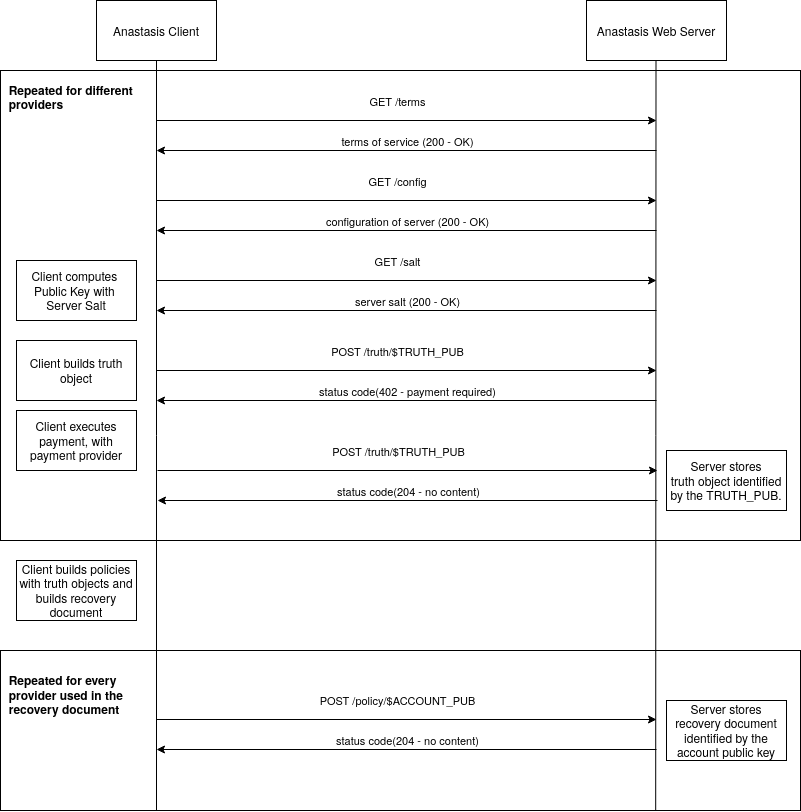
\includegraphics[scale=0.5]{images/secret_split.png}
	\caption{Secret split process}
	\label{fig:secret_split}
\end{figure}
\newpage
\begin{enumerate}
\item The user selects a new escrow provider on which per wants to
  store a truth object.
\item The client software downloads the terms of service for this
  provider (GET /terms). This is also a check if the server is
  available if this command doesn't respond the client will abort the
  process.
\item Next the client requests the server configuration (GET
  /configuration). The configuration lists the available
  authentication methods and the protocol version of the server.
\item The client downloads the server salt (GET /salt). The salt is
  used to generate the server specific account public key, which
  identifies the user.
\item After the user has generated the public key, per will create a
  truth object on the client. The truth object contains all the needed
  information for the recovery for this key share. This truth object
  is sent encrypted to the server and stored under the TRUTH\_PUB the client
  generated (POST /truth/\$TRUTH\_PUB).
\item In this scenario the client has not jet paid for the
  upload. This means the server will respond with the HTTP status code
  \texttt{402 Payment required}. The client first must do a payment with our
  payment provider --- GNU Taler. After the successful payment the client
  will receive a payment identifier. With this payment identifier he
  can resend the previously failed request.
\item The user will now repeat the steps 1-6 until per thinks that they
  have setup a sufficient amount of authentication methods. The user
  can now combine these providers to create policies. For example per
  may have stored three truth objects at three different providers.
  This means per can now define combinations with these providers,
  for example A+B, A+C and B+C. This means the user has three ways to
  recover their secret.
\item After the user has generated the policies the client will
  generate a recovery document. The recovery document contains a list
  of all truth\_seed's used, a list of the policies and the encrypted core
  secret of the user. The client will now send a encrypted recovery
  document to each provider used in the recovery document (POST
  /policy/\$ACCOUNT\_PUB). Through this, the recovery document is
  replicated and recovery can proceed without a single point of
  failure.
\end{enumerate}
\newpage
\subsubsection{Secret recovery}

Figure~\ref{fig:recovery_process} illustrates the recovery process.
\begin{figure}[H]
	\centering
		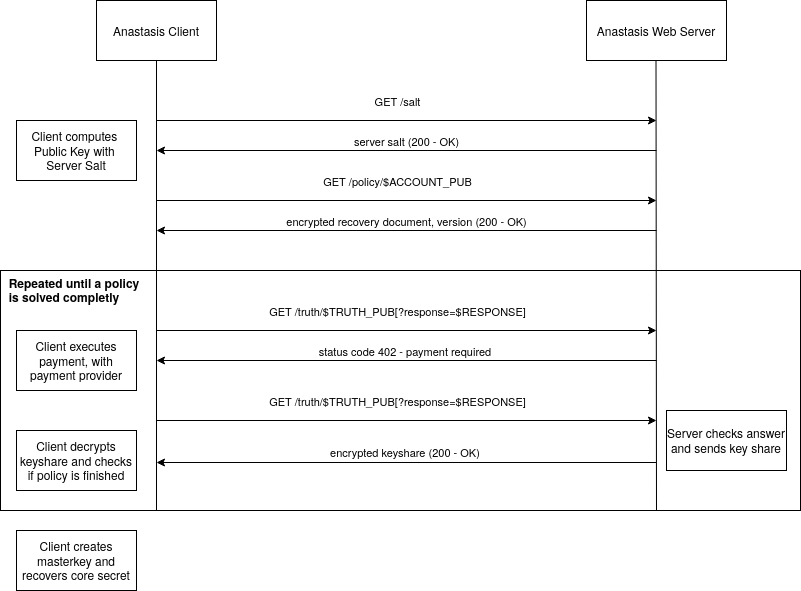
\includegraphics[scale=0.5]{images/recovery_process.png}
	\caption{Secret recovery process}
	\label{fig:recovery_process}
\end{figure}
\begin{enumerate}
\item The user selects a server on which per previously stored a
  recovery document.
\item Next the client downloads the server salt to compute the server
  specific account public key (GET /salt).
\item After the user generated the public key, per will download the
  recovery document. At this point per can define a
  specific version or the latest version of the recovery document. In
  the illustration the client downloads the latest version (GET
  /policy/\$ACCOUNT\_PUB).
\item The client will now decrypt the recovery document and list all
  policies and authentication methods. The user now has to solve these
  challenges. In this example the user has to answer a secure question
  which was sent to them in the recovery document. (GET
  /truth/\$TRUTH\_PUB?response=\$RESPONSE) \\
\item Note the server can define that a challenge has a certain cost,
  in this scenario the server rejects the first request because the
  user has not yet paid for recovery.  After the payment the user can
  resend the request.  After each successfully solved challenge the
  client will check if one of the policies is completely satisfied.
  If all shares needed for one of the policies have been recovered,
  the client will decrypt the core secret and provide it to the user.
\end{enumerate}

Figure~\ref{fig:recovery_process} shows the flow using a secure
question for the authentication challenge. If the user would have
chosen a complex authentication method like SMS or E-Mail, the client
would first need to start the challenge with the request (GET
/truth/\$TRUTH\_PUB). The server would then notify the user that per will
receive some token out of bounds. After that, the user would have to
provide for example the PIN sent to them via SMS with the same request
as before (GET /truth/\$TRUTH\_PUB?response=\$RESPONSE).


\subsection{Client Application Command Line Interface (CLI)}

There are two client applications which interact with the user. First
the Anastasis {\em splitter} and second the Anastasis {\em
  assembler}. The splitter application is responsible for the backup
of the core secret. The assembler is then responsible for the recovery
of the core secret.

Both commands are started with a configuration option ``--me=FILE''
that gives the name of a file with the user's identity attributes.

\subsubsection{Anastasis splitter}

The user starts the assembler by passing a JSON document with their
unforgettable identity attributes (name, social security number, ...).

The following commands are available:

\begin{itemize}
\item server add \$URL: this command lets the user add escrow
  providers. The command will check if a supported escrow service is
  available under the provided URL. Afterwards it will download its
  terms and salt. The server needs to be added before the user can do
  any uploads on it.
\item truth add \$server \$method \$truth: with this command the user
  can upload a truth on a previously added server. The user needs to
  specify the authorization method used and the truth for the
  authorization process, for example the phone number for SMS
  authentication.  The application will check if the server supports the
  provided method before uploading.
\item policy add \$truth1 \$truth2...: after a user has added all the
  truths, per can start to create policies. Per can combine the truths
  in any way they wish. It is also possible to just store one truth in
  a policy, but this is not recommended since it defies the design of
  the application.
\item policy: shows all created policies.
\item truth: shows all created truths.
\item server: shows all added servers.
\item publish \$secret: if the user is finished per can publish the
  configuration. The application will then generate the recovery
  document with the provided information and secret. Afterwards, it
  will upload the recovery document on every server that was used. For
  recovery, the user only needs to remember any one of the servers.
\end{itemize}

Below is an example transcript of an interaction with the splitter:

\begin{lstlisting}
$ anastasis-splitter --me=identity.json
anastasis-splitter> server add $URL1
version: 1.0
annual fee: 4.99 KUDOS,
available policy methods: sms
Server #1 available
anastasis-splitter> server add $URL2
version: 1.0
annual fee: 3.99 KUDOS,
available policy methods: sms, question
Server #2 available
anastasis-splitter> truth add server#1 sms +492452526
Truth #1 added for server #1
anastasis-splitter> truth add server#2 mail "hoehenweg 80, Biel"
Sorry, server #2 does not support 'mail'
anastasis-splitter> truth add question "favorite color" "red"
Truth #2 added
anastasis-splitter> policy add truth#1 truth#2
Policy #1 defined
anastasis-splitter> policy
Policy#1: #truth#1 #truth2
anastasis-splitter> truth
truth#1: server#1 sms  +492452526
truth#2: server#2 question "favorite color" <OMITTED>
anastasis-splitter> truth --secrets
truth#1: sms  +492452526
truth#2: question "favorite color" "red"
anastasis-splitter> server
server#1: http://anastasis.example.com/ methods: sms,
insured up to: 420 KUDOS, cost: 0.4 KUDOS
anastasis-splitter> publish
Server#1 failure: 402 payment required:
payto://pay/ABALSASDFA KUDOS:0.3
Server#2 failure: 402 payment required:
payto://pay/ABALSAADAS KUDOS:0.5
Total: 0.8 KUDOS
# Here: taler-wallet-cli payto://pay/ABALASDFA used to pay!
anastasis-splitter> publish
Server#2 failure: 402 payment required
# Here: taler-wallet-cli payto://pay/ABASDFASDF used to pay!
anastasis-splitter> publish "my super secret"
Thank you for using Anastasis.
$
\end{lstlisting}

\subsubsection{Anastasis assembler}

The user starts the assembler by passing a JSON document with their
unforgettable identity attributes (name, social security number, ...).
They also must pass the URL of an escrow provider which stores their
recovery document, as well as the requested version of the recovery
document. The assembler will then download and decrypt the recovery
document and begin the recovery process.


The following commands are available:
\begin{itemize}
\item truth: shows all available authorization challenges
  from the recovery document and their status (``(-)'' not solved, ``(+)'' solved)
\item policies: shows all available policies in the recovery document and
  the respective status of the truths used in each policy.
\item try \$truth: this command starts an authorization process which
  needs interaction with external services like SMS or email. It shows
  the instructions to follow to authorize release of the share.
\item answer \$truth \$answer: this command tries to answer the
  selected challenge with the provided answer. The application will
  check the answer and give a feedback to the user. Every time a
  challenge is solved, the client API will check if as a result any of
  the policies is completely satisfied.  If any policy was completely
  satisfied, the assembler will print out the recovered core secret
  and exit.
\end{itemize}

Below is an example transcript of an interaction with the assembler:

\begin{lstlisting}
$ anastasis-assembler --import https://anastasis.example.com/
--policy-version=42 --me=identity.json
anastasis-assembler> truth
truth#1(-): KUDOS 0.0 question "favorite color"
truth#2(-): KUDOS 0.4 sms
truth#3(-): KUDOS 2.6 post
anastasis-assembler> policies
policy#1: KUDOS 0.4 truth#1 truth#2 missing
policy#2: KUDOS 3.0 truth#1 truth#2 truth#3 missing
anastasis-assembler> try truth#2
payto://pay/BASDFASD
# SMS arrives asynchronously
anastasis-assembler> answer truth#2 1234
Success truth#2
anastasis-assembler> answer truth#1 "blue"
Failed truth#1
anastasis-assembler> truth
truth#1(-): KUDOS 0.0 question "favorite color"
truth#2(+): KUDOS 0.4 sms
truth#3(-): KUDOS 2.6 post
anastasis-assembler> policies
policy#1: KUDOS 0.0 truth#1 missing
policy#2: KUDOS 2.6 truth#1 truth#3 missing
anastasis-assembler> answer truth#2 "red"
Success truth#2
//One of the policies was solved successfully and the secret is recovered.
Secret was: "my super secret"
$
\end{lstlisting}



\subsection{Libraries} \label{sec:libraries}

In this section the libraries used by Anastasis are presented.

\subsubsection{GNU Taler}

GNU Taler is one of the main reasons why we started to implement
Anastasis, since the application needs a system to back up the private
keys of their users.  ``GNU Taler is a privacy-preserving payment
system. Customers can stay anonymous, but merchants can not hide their
income through payments with GNU Taler. This helps to avoid tax
evasion and money laundering.''~\cite{gnu_taler}

To operate GNU Taler the user needs to install an electronic
wallet. Backups of the wallet are secured with a secret key. Here
comes Anastasis into play, Anastasis will secure this secret key for
the user.

In our implementation GNU Taler is also our payment system. We decided
to use GNU Taler because both Anastasis and GNU Taler are privacy
preserving applications. If we for example used credit cards for
payments the user would no longer be anonymous which is helpful for
the security of Anastasis as it allows us to use the user's name in
the user's identity attributes.  GNU Taler is also a GNU package
and Free Software.~\cite{gnu_taler}
\newpage
\subsubsection{PostgreSQL}

PostgreSQL is a Free/Libre Open Source object-relational
database. PostgreSQL has over 30 years of active development which
makes it a stable and reliable software.

We use PostgreSQL as our database on the Anastasis server. We decided
to use PostgreSQL because it is an open source and lightweight
software which has a big community.  This means there are a lot of
helpful documentations and forums.~\cite{postgresql}

\subsubsection{Libcurl}

Libcurl is a libre URL transfer library. Libcurl supports a wide range
of protocols and a C API. Libcurl is also ready for IPv6 and SSL
certificates.

For Anastasis we use Libcurl to generate the client-side HTTP
requests. We decided to use Libcurl because it is also written in C
and free software. The software is also well supported and has a good
documentation.  This makes the integration in our application
easy.~\cite{libcurl}

\subsubsection{GNU Libmicrohttpd}

GNU libmicrottpd is a small C library which provides an easy way to
run a HTTP server.  We use GNU Libmicrohttpd in Anastasis to provide a
simple webserver. The main reason why we did not use apache or nginx
is that we do not need a standalone webserver. The Anastasis webserver
just must handle some API requests, a standalone webserver is not
needed for that and would make the infrastructure more complex to
maintain and develop.  GNU Libmicrohttpd is also a GNU package
and Free Software.~\cite{libmicrohttpd}

\subsection{Testing}

To test our application, we used the GNU Taler testing library as our
foundation for t of our testings.  This library allows you to create testing instances of
both the Anastasis application and the GNU Taler payment system. We
implemented unit tests for the crypto functions and the database operations.
The following four tests are independently performed.

\begin{itemize}
\item The first test is the database test. The Anastasis testing library first connects to a test database, this database is only used for the testing, we never test on the live database. The test first deletes and recreates the database. After that it will perform several unit tests to check if the database queries of the application are working as intended.
\item Next we test the Anastasis crypto API, it tests all the
cryptographic functions used in the API with unit tests.
The most important part is  that the recreation of the keys
and decryption works as intended.
\item After the basic parts of the application are tested the client
will test every request in the Anastasis server API. For this we need the
Taler Testing library. The Taler testing library will start an instance
of the Anastasis webserver and a GNU Taler merchant service. The merchant
service is needed to process the payment operations. The testing library
will now send a request to every end point of the Anastasis REST API. It will
check if every response of the REST API is as intended.
\item At the end the whole application flow is tested. For this
we need to start a Anastasis server, Taler merchant and Taler exchange instance.
The library will now perform a full secret split and secret recovery.
This test is successful if the provided core secret at the begin, matches the
recovered core secret.
\end{itemize}
